\documentclass{note}
\usepackage[cpp,table,pseudo]{mypackage}
\usepackage{footnote}
\makesavenoteenv{tabular}

\renewcommand{\thefootnote}{\fnsymbol{footnote}}
\newenvironment{bayesian}{\begin{center}\begin{tikzcd}[cells={nodes={draw=black, circle}}]}{\end{tikzcd}\end{center}}

\def\Ent{\mathrm{Ent}}

\title{人工智能笔记}
\author{陈鸿峥}
\date{{\builddatemonth\today}\protect\footnote{\text{Build \builddate\today}}} % protect!

\begin{document}

\maketitle
\renewcommand{\thefootnote}{\arabic{footnote}}
\setcounter{footnote}{0}

\setcounter{tocdepth}{2}%设置深度
\tableofcontents

\bigskip\bigskip

% !TEX root = main.tex

\section{计算机系统概述}
\subsection{计算模型}
\begin{itemize}
	\item 图灵机(1936)
	\item 冯诺依曼体系结构(1945)\footnote{非冯诺依曼体系结构:并行计算、量子计算、生物计算} --- 存储程序原理(\textbf{运算器}为中心)\\
	计算机采用\textbf{二进制}表示机器指令和数据,按照程序指令\textbf{顺序}执行
\begin{center}
\begin{tikzcd}
& & \text{存储器}\arrow{d} & & \\
\quad\arrow{r} & \text{输入设备}\arrow{r} & \text{运算器}\arrow{r}\arrow{d}\arrow{u} & \text{输出设备}\arrow{r} & \quad\\
& & \text{控制器}\arrow{u}\arrow{lu}\arrow{ru}\arrow[bend left]{uu} & &
\end{tikzcd}
\end{center}
而现在由于计算不是瓶颈,存储访问成为了瓶颈,故现代微机以\textbf{存储器}为中心
\begin{center}
\begin{tikzcd}
& & \text{运算器}\arrow{d} & & \\
\quad\arrow{r} & \text{输入设备}\arrow{r} & \text{存储器}\arrow{r}\arrow{d}\arrow{u} & \text{输出设备}\arrow{r} & \quad\\
& & \text{控制器}\arrow{u}\arrow{lu}\arrow{ru}\arrow[bend left]{uu} & &
\end{tikzcd}
\end{center}
\end{itemize}
[运算器、控制器](CPU)、存储器为计算机的核心,合称主机;外围设备,简称外设,指除主机外的其他设备,包括IO设备、外存等

计算机中的信息仍用二进制表示的原因:由物理器件性能决定
\begin{itemize}
	\item 二进制只有两种状态,容易找到具有2个稳定状态并且状态转换容易控制的物理器件(数字电路)
	\item 二进制编码运算规则简单
	\item 二进制的0、1与二值逻辑一致,容易实现逻辑运算
\end{itemize}
% There are two reasons computers use the binary system:
% 1.Two clearly distinct states that provide a safety range for reliability.
% 2.Least amount of necessary circuitry, which results in the least amount of space, energy consumption, and cost.

\subsection{计算机的发展历程}
按发展历程可分为:电子管、晶体管、集成电路、(超)大规模集成电路四代计算机
\par重大历史事件如下
\begin{center}
\begin{tabular}{|c|c|c|c|}
\hline
% 年份 & 姓名 & 事件 & 备注 \\
1904 & 弗莱明(Fleming) & 二极管 & \\\hline
1907 & 德福雷斯特(De Forest) & 三极管 & \\\hline
1938 & 香农(Shannon) & 布尔代数与二值电子器件(继电器) & 奠定数字电路基石 \\\hline
1946 & & 第一台通用计算机ENIAC & 十进制 \\\hline
1947 & \begin{tabular}{c}布莱顿(Brattain)\\
巴丁(Bardeen)\end{tabular} & 点接触晶体管 & \\\hline
1949 & 肖克利(Shockley) & 结型晶体管(1949) & 1956诺贝尔奖\\\hline
1950 & & 二进制和存储程序EDVAC & 实现冯诺依曼设想(组合进步) \\\hline
1958 & Jack Kilby & 集成电路 & 2000诺贝尔奖 \\\hline
1965 & Moore & 摩尔定律 & \begin{tabular}{c}
在价格不变的情况下,每18个月芯片上\\
晶体管数目翻倍,性能也提升一倍
\end{tabular}\\\hline
1971 & Intel & 第一款微处理器4004 & 10$\mu$m\\\hline
\end{tabular}
\end{center}

\subsubsection{单处理器(1971-2002)}
性能提升主要手段
\begin{itemize}
	\item 提升工作主频:KHz增长至GHz(生产工艺进步,流水线级数增加)
	\item 指令级并行(ILP)
\end{itemize}
\begin{proposition}[安迪-比尔定律]
Andy gives, Bill takes away. 安迪是原Intel CEO,比尔是原微软CEO,硬件厂商靠软件开发商用光自己提供的硬件资源得以生存
\end{proposition}
但遇到频率墙和功耗墙
\[\text{功耗(power)}\propto 1/2\times\text{CMOS电容}\times\text{电压}^2\times\text{转换(01)频率}\]
\par
2004年,Intel放弃4GHz Pentium4芯片开发,因无法解决散热问题,通过加快主频提升处理器性能的路走到尽头

\subsubsection{多核处理器(2005-)}
采用多核处理器不过是将硬件的问题丢到软件\footnote{“向多核的转变并不是因为我们在软件或体系结构技术上取得了中大突破而带来的。相反,这种转变是当单处理器体系结构发展遇到了难以克服的巨大障碍时,我们被迫作出的一种选择。”---Kurt Keutzer (UCB), \emph{The Landscape of Parallel Computing Research: A View from Berkeley}}
\begin{theorem}[阿姆达尔(Amdahl)定律]
\label{thm:amdahl}
\[\text{改进后的执行时间}=\text{受改进影响部分的执行时间}/\text{改进提高的倍数}+\text{不受影响的执行时间}\]
\[S_A=\frac{1}{s+(1-s)/N},\]
\end{theorem}
对计算机系统的某个部分采用并行优化措施后所获得的计算机性能的提高是有上限的,上限由串行部分所占的比例决定
\begin{theorem}[古斯塔夫森(Gustafson)定律]
\[S_G=(s'+p'\times N)/(s'+p')=N+(1-N)\times s',\]
其中,$s'$和$p'$为程序串行部分与可并行化部分在并行系统上执行的时间占总时间的比例,$N$为处理器数量,简便起见设总时间$s'+p'=1$
\end{theorem}
打破Amdahl定律\textbf{问题规模不变}的假设,任何足够大的任务都可以被有效地并行化,只要问题规模可扩展,并行所带来的加速比就可以扩展


\subsection{计算机系统的层次结构}
\begin{center}
\begin{tikzcd}
\text{高级语言层}\arrow{d}{}\\
\text{汇编语言层}\arrow{d}{}\\
\text{操作系统层}\arrow{d}{}\\
\text{指令系统层}\arrow{d}{}\\
\text{微体系结构层}\arrow{d}{}\\
\text{数字逻辑层}
\end{tikzcd}
\end{center}
程序编译运行过程:
\begin{center}
\begin{tikzcd}
\text{高级语言}\quad\arrow{r}{\text{预编译、编译}} & \quad\text{汇编语言}\arrow{r}{\text{汇编}} & \text{目标文件(二进制)}\arrow{r}{\text{链接}} & \text{可执行文件(二进制)}\arrow{d}{\text{加载}}\\
& & \text{电路上的电信号}\quad & \quad\text{二进制机器指令流(硬盘$\to$存储器)}\arrow[swap]{l}{\text{CPU取指译码}}
\end{tikzcd}
\end{center}
计算机内部工作过程:逐条执行加载到内存中的二进制机器指令流的过程

指令执行分为两个阶段,周期性重复性进行:
\begin{itemize}
	\item 取指阶段:CPU从内存中读取指令,程序计数器(PC)保存要被要被取出的\textbf{下一条}指令的地址,除非遇跳转指令,否则都加一个增量\footnote{程序计数器(Program Counter)是一个实际存在的寄存器吗? - Belleve的回答 - 知乎 \url{https://www.zhihu.com/question/22609253/answer/21965180} PC每次增加\textbf{一条指令的长度/寻址粒度},在MIPS中一条指令长4字节,寻址粒度1字节,故每次PC加4;而x86体系指令长度不定,每次增加量会变化}
	\item 执行阶段:对取出的指令译码后执行
\end{itemize}
软件系统可分为系统软件和应用软件

\subsection{计算机结构的八个想法}
\begin{enumerate}
	\item 摩尔(Moore)定律:集成电路资源每$18-24$个月翻倍
	\item 抽象(abstraction):简化设计
	\item 加速常用操作(Make common case fast):见定理\ref{thm:amdahl}
	\item 并行(parallelism)
	\item 流水线(pipelining)
	\item 预测(prediction)
	\item 内存等级制(hierarchy)
	\item 冗余实现可靠性(redundancy):检测故障及解决
\end{enumerate}

\subsection{基本指标}
表示计算机通信带宽时
\begin{center}
\begin{tabular}{ccccccc}\hline
KB(yte) & MB & GB & TB & PB & EB & ZB\\\hline
$10^3$ & $10^6$ & $10^9$ & $10^{12}$ & $10^{15}$ & $10^{18}$ & $10^{21}$\\\hline
\end{tabular}
\end{center}
表示计算机存储二进制时
\begin{center}
\begin{tabular}{ccccccc}\hline
KiB(yte) & MiB & GiB & TiB\\\hline
$2^{10}$ & $2^{20}$ & $2^{30}$ & $2^{40}$\\\hline
\end{tabular}
\end{center}
\begin{itemize}
	\item 位(bit/b):计算机处理、存储、传输信息的最小单位
	\item 字节(Byte/B) $1\text{ Byte}=8\text{ bit}$:现代计算机主存按字节编制,字节是最小可寻址单位
	\item 字(Word):表示被处理信息的单位,用来度量数据类型的宽度\footnote{字长是指CPU中\textbf{数据通路的宽度},等于CPU内部总线的宽度或运算器的位数或通用寄存器的宽度;字和字长的宽度可以一样,也可以不同,通常是字节的整数倍}
\end{itemize}
\par 一台32位的电脑,一个字等于4个字节,字长为32位;若字长为16位,则一个字等于2字节.
\par 4字节相当于8位16进制编码

\subsection{性能评价}
\label{subsec:performance}
CPU主频:对同一型号计算机,主频越高,完成指令一个执行步骤时间越短
\[\text{计算机的性能(Performance)}=1/\text{执行时间(Execution time)}\]
按照单位(量纲)进行换算即可
\[\begin{aligned}
\text{CPU执行时间(s)}&=\text{执行程序所需CPU时钟周期(cyc)}\times\text{时钟周期s/cyc)}\\
&=\text{指令数目(ins)}\times\text{CPI(cyc/ins)}\times\text{时钟周期(s/cyc)}
\end{aligned}\]
程序性能对执行事件的影响:
\begin{center}
\begin{tabular}{|c|c|c|c|}\hline
 & 指令数 & CPI & 时钟周期\\\hline
算法、编程语言、编译器 & $\times$ & $\times$ & \\\hline
指令集 & $\times$ & $\times$ & $\times$ \\\hline
计算机组成 & & $\times$ & $\times$ \\\hline
实现技术 & & & $\times$\\\hline
\end{tabular}
\end{center}
体系结构=指令集体系结构(功能定义与设计)+计算机组成(考虑用什么材料)\\
举例来说:
\begin{itemize}
	\item 指令集(ISA)考虑:是否提供乘法指令
	\item 组成(Organization)考虑:如何实现乘法指令(专门乘法器还是加法器+移位器)
	\item 实现技术(Technology)考虑:如何布线、用什么材料和工艺
\end{itemize}

% 带有处理器的设备一般称为智能化设备
% 完整的计算机系统应包括配套的硬件设备和软件系统
% !TEX root = main.tex

\section{搜索}
% Problem solving by search: formalization
% Uninformed search: Breadth-First, Uniform-Cost, Depth-First, Depth-Limited, and Iterative- Deepening
% Heuristic search: Greedy best-first, A*
% Properties of search: completeness, optimality, time and space complexity
% Path/cycle checking
% Game tree search: MiniMax, alpha-beta pruning
% CSP: Formalization, backtracking, forward checking, and GAC algorithms

搜索主要包括无信息(uninformed)搜索和有信息搜索。
\begin{itemize}
	\item 状态空间(state space)
	\begin{itemize}
		\item 传统搜索:状态空间可见、动作确定性
		\item 非传统搜索:局部搜索、模拟退火、爬坡
	\end{itemize}
	\item 动作(action):不同状态之间的转换
	\item 初始状态(initial state)
	\item 目标/期望(goal)
\end{itemize}
% 对抗搜索(adversarial):博弈树(minimax)、$\alpha-\beta$剪枝

树搜索,边界集(frontier)是未探索的状态集合
\begin{algorithm}[H]
\caption{Tree Search}
\begin{algorithmic}[1]
\Procedure{TreeSearch}{(Frontier, Successors, Goal?)}
\If{Frontier is empty}
\State \Return failure
\EndIf
\State Curr $=$ select state from Frontier
\If{Goal?(Curr)}
\State \Return Curr
\EndIf
\State $\text{Frontier'} = (\text{Frontier} - \{\text{Curr}\}) \cup \text{Successors(Curr)}$
\State \Return TreeSearch(Frontier',Successors,Goal?)
\EndProcedure
\end{algorithmic}
\end{algorithm}

搜索需要关注的几个特性:
\begin{itemize}
	\item 完备性:若解存在,搜索是否总能找到解
	\item 最优性:是否总能找到最小代价的解
	\item 时间复杂性:最大需要被\textbf{生成或展开}\footnote{而不是探索的结点数目}的结点数
	\item 空间复杂性:最大需要被存储在内存中的结点数
\end{itemize}

\subsection{无信息搜索}
无信息搜索并不考虑关于特定搜索问题的领域特定的信息,主要包括宽度优先、一致代价、深度优先、深度受限、迭代加深五种算法。

\subsubsection{宽度优先搜索(BFS)}
将后继加入边界集的\textbf{后面},$b$为最大状态后继数目/分支因子(branching factor),$d$为最短距离解的行动数(注意是\textbf{边数},而不是层数!)
\begin{itemize}
	\item 完备性与最优性:所有短路总在长路前被探索,某一长度只有有限多条路径,最终可以检测所有长度为$d$的路径,从而找到最优解
	\item 时间复杂度:$1+b+b^2+\cdots+b^d+(b^d-1)b=O(b^{d+1})$,最差情况在最后一层的最后一个节点才探索到最优解,从而前面$b$个节点都要展开第$d+1$层
	\item 空间复杂度:$b(b^d-1)=O(b^{d+1})$,需要将边界集都存储下来,同上最后一层
\end{itemize}

\subsubsection{深度优先搜索(DFS)}
将后继加入边界集的\textbf{前面},即总是展开边界集中最深的节点
\begin{itemize}
	\item 完备性
	\begin{itemize}
		\item 无限状态空间:不能保证
		\item 有限状态空间无限路径:不能保证(可能有环)
		\item 有限状态空间+路径/重复状态剪枝:可以保证
	\end{itemize}
	\item 最优性:因完备性不能保证,故最优性也不能保证
	\item 时间复杂性:$O(b^m)$,其中$m$为状态空间的最长路的长度(若$m>>d$,则非常糟糕;但如果有大量解路径,则会快于BFS)
	\item 空间复杂性:$O(bm)$,\textbf{线性空间复杂性}是DFS最大的优点。边界集只包含当前路径的最深节点以及回溯节点(backtrack points为当前路径上节点的未探索的兄弟sibling)。
	注意这里需要记录路径上每个结点的孩子,因已被扩展。
\end{itemize}

\subsubsection{一致代价(Uniform-cost)}
一致代价搜索(Uniform cost search, UCS)\footnote{至于为什么叫Uniform,可以看\url{https://math.stackexchange.com/questions/112734/in-what-sense-is-uniform-cost-search-uniform}和\url{https://cs.stackexchange.com/questions/6072/why-is-uniform-cost-search-called-uniform-cost-search},比较合理的解释是到达同一结点的cost都被认为是相同的(寻找最优解时)。一致的算法总是选择边界集中第一个元素。}的边界集以路径开销升序排序,总是先展开最低开销的路径。
如果每一个动作都是一样的代价,则一致代价等价于BFS。
\begin{itemize}
	\item 完备性与最优性:假设所有转移都有代价$\geq\eps>0$,所有更低代价的路径都在高代价路径之前被展开,只有有限多的路径开销小于最优解的开销,故最终一定会到达最优解
	\item 时间复杂性:$O(b^{\lfloor C^\star/\eps\rfloor+1})$,对应着BFS中$d=C^\star/\eps$,其中$C^\star$为最优解的开销,最坏情况就是每一层开销都很小为$\eps$,那么需要$\lfloor C^\star/\eps\rfloor$层
	\item 空间复杂性:$O(b^{\lfloor C^\star/\eps\rfloor+1})$
\end{itemize}

\subsubsection{深度受限搜索(Depth-limited)}
只在最大深度执行DFS,因此无穷路径长不会存在问题
\begin{itemize}
	\item 完备性与最优性:不能保证,若解的深度大于$L$
	\item 时间复杂度:$O(b^L)$
	\item 空间复杂度:$O(bL)$
\end{itemize}

\subsubsection{迭代加深搜索(Iterative Deepening)}
IDS逐渐增加最大深度$L$,对每一个$L$做深度受限搜索
\begin{itemize}
	\item 完备性:可以保证
	\item 最优性:如果开销一致\footnote{若开销不一致,则可以采用代价界(cost bound)来代替:仅仅展开那些路径开销小于代价界的路径,同时要记录每一层深搜的最小代价。这种方式的搜索开销会非常大,有多少种不同路径开销就需要多少次迭代循环。},则可以保证
	\item 时间复杂性:$(d+1)b^0+db+(d-1)b^2+\cdots+b^d=O(b^d)$,第$0$层搜了$(d+1)$次,以此类推。可以看到时间复杂度是\textbf{比BFS优}的,因为最后一层的结点并未进行展开。
	\item 空间复杂性:$O(bd)$,同DFS
\end{itemize}

\subsubsection{双向搜索(Bidirectional)}
从源结点和汇结点同时采用BFS,直到两个方向的搜索汇聚到中间。
\begin{itemize}
	\item 完备性:由BFS保证
	\item 最优性:若一致代价则可保证
	\item 时间复杂性:$O(b^{d/2})$
	\item 空间复杂性:$O(b^{d/2})$
\end{itemize}

\subsubsection{环路/路径检测}
所有检测都是在\textbf{扩展时}进行:
\begin{itemize}
	\item 环路(cycle)检测:检测当前状态是否与所有已探索的状态重复(BFS)
	\item 路径(path)检测:只检测当前状态是否与该路径上的状态重复(DFS)
\end{itemize}
注意不能将环路检测运用在BFS上,因为这会破坏其空间复杂度的优势。

环路检测运用到UCS上依然\textbf{可以保证最优性}\footnote{注意这在启发式搜索中不一定成立}。
因为UCS第一次探索到某一状态的时候已经发现最小代价路径,因而再次探索该状态不会发现路径比原有的更小。

\subsubsection{总结}
\begin{center}
\begin{tabular}{ccccccc}\hline
& BFS & UCS & DFS & Depth-limited & IDS & Bidirectional\\\hline
完备性 & \cmark & \cmark & \xmark & \xmark & \cmark & \cmark\\
时间复杂度 & $O(b^d)$ & $O(b^{\lfloor C^\star/\eps\rfloor+1})$ & $O(b^m)$ & $O(b^l)$ & $O(b^d)$ & $O(b^{d/2})$\\
空间复杂度 & $O(b^d)$ & $O(b^{\lfloor C^\star/\eps\rfloor+1})$ & $O(bm)$ & $O(bl)$ & $O(bd)$ & $O(b^{d/2})$\\ 
最优性 & \cmark & \cmark & \xmark & \xmark & \cmark & \cmark\\\hline
\end{tabular}
\end{center}

\begin{example}
$N$个传教士和$N$个食人族要过河,他们都在河的左岸。
现在只有一条船能够运载$K$个人,要把他们都运往右岸。
要满足无论何时何地,传教士的数目都得大于等于食人族的数目,或者传教士数目为0。
\end{example}
\begin{analysis}
考虑对问题形式化为搜索问题
\begin{itemize}
	\item 状态$(M,C,B)$,其中$M$为左岸传教士数目,$C$为左岸食人族数目,$B=1$指船在左岸
	\item 动作$(m,c)$指运$m$个传教士和$c$个食人族到对岸
	\item 先决条件:传教士数目和食人族数目满足限制
	\item 效果:$(M,C,1)\stackrel{(m,c)}{\implies}(M-m,C-c,0)$\\
	$(M,C,0)\stackrel{(m,c)}{\implies}(M+m,C+c,1)$
\end{itemize}
\end{analysis}
% !TEX root = main.tex

\subsection{有信息搜索}
% Heuristic search: Greedy best-first, A*

在无信息搜索中,我们从不估计边界集中最有期望(promising)获得最优解的结点,而是无区别地选择当前边界集中第一个结点。
然而事实上,针对不同问题我们是有对结点的先验知识(apriori knowledge)的,即从当前结点到目标结点的开销有多大。
而这就是有信息搜索(informed),或者称为启发式搜索(heuristics)。

关键在于领域特定启发式函数$h(n)$的设计,它估计了\textbf{从结点$n$到目标结点的开销(cost)}。
注意满足目标状态的结点$h(n)=0$。

\subsubsection{贪心最优搜索(Greedy Best-First Search)}
直接使用$h(n)$对边界集进行排序,但这会导致贪心地选择\textbf{看上去}离目标结点开销最小的路径。

如果存在环路,贪心最优搜索是不完备的,会陷入死循环。
\begin{center}
\begin{tikzcd}
 & s\arrow[ld]\arrow[rd] &\\
n_1\arrow[bend right,d] & & n_3\arrow[d]\\
n_2\arrow[bend right,u] & & \text{Goal}
\end{tikzcd}
\end{center}

\subsubsection{A$^\star$搜索}
综合考虑当前已走的开销和未来估计的开销。
定义一个估值函数
\[f(n)=g(n)+h(n)\]
其中$g(n)$为路径到节点$n$的代价,$h(n)$为从$n$到目标节点的代价,采用$f(n)$对边界集内的节点进行排序。
\textemph{当$f(n)$相同时,再用$h(n)$进行升序排序。}

$f(n)$需要满足下列两个性质。
\begin{definition}[可采纳的(admissibility)]
假设所有代价$c(n1\to n2)\geq\eps>0$,令$h^\star(n)$为从节点$n$到目标节点$\infty$的最优解代价\footnote{如果没有路径则$h^\star(n)=\infty$},若
\[\forall n:\;h(n)\leq h^\star(n)\]
则称$h(n)$是可采纳的。
即一个可采纳的启发式函数总是\textemph{低估}了当前结点到目标结点的真实开销(这样才能保证最优解不被排除)。
因此对于任何目标结点$g$都有$h(g)=0$。
\end{definition}
\begin{definition}[一致性(consistency)/单调性(monotonicity)]
若对于所有的结点$n_1$和$n_2$,$h(n)$满足(三角不等式)
\[h(n_1)\leq c(n_1\to n_2)+h(n_2)\]
则称$h(n)$是单调的。
\end{definition}

\begin{theorem}
一致性蕴含可采纳性
\end{theorem}
\begin{analysis}
分类讨论
\begin{itemize}
	\item 当结点$n$没有到目标结点的路径,则$h(n)\leq h^\star(n)=\infty$恒成立
	\item 令$n=n_1\to n_2\to\cdots\to n_k$为从结点$n$到目标结点的最优路径,则可以用数学归纳法证明$\forall i:\;h(n_i)\leq h^\star(n_i)$,如下从后往前推
	\[h(n_{i})\leq c(n_i\to n_{i+1})+h(n_{i+1})\leq c(n_i\to n_{i+1}) + h^\star(n_{i+1})=h^\star(n_i)\]
\end{itemize}
\end{analysis}

\begin{theorem}
可采纳性蕴含最优性
\end{theorem}
\begin{analysis}
假设最优解有开销$C^\star$,则任何最优解一定会在开销大于$C^\star$的路径之前被展开(有限条路径)。

反证若路径$p$的代价$c(p)$大于最优解路径代价$c(p^\star)$且$p$在$p^\star$之前被扩展,则一定存在一个节点$n$在$p^\star$上且仍在边界集中,因此
\[c(p)\leq f(p)\leq f(n)=g(n)+h(n)\leq g(n)+h^\star(n)=c(p^\star)\]
矛盾。故在最优解展开之前的路径一定有开销$\leq C^\star$,最终我们一定会检测到最优解,而且次优解不会在最优解之前被检测。
\end{analysis}

做环检测可能导致找不到最优解。
可采纳性不能保证最优解,但\textemph{单调性环检测保证最优解}。

单调性有以下几个性质
\begin{proposition}
路径上的$f$一定是非递减的
\end{proposition}
\begin{analysis}
\[\begin{aligned}
f(n)&=g(n)+h(n)\\
&\leq g(n)+c(n\to n')+h(n')\\
&= g(n')+h(n')\\
&= f(n')
\end{aligned}\]
\end{analysis}
\begin{proposition}
如果$n_2$在$n_1$之后被扩展,则$f(n_1)\leq f(n_2)$
\end{proposition}
\begin{proposition}
当$n$在任何小于$f$值得路径之前被展开
\end{proposition}
\begin{proposition}
$A^\star$算法第一次展开某个状态时,它已经找到了到达那个状态的最小开销路径。
\end{proposition}

\subsubsection{迭代加深A$^\star$(IDA)算法}
$A^\star$算法有和BFS或UCS同样的空间复杂性问题,而迭代加深$A^\star$算法同样解决空间复杂度的问题。
与迭代加深类似,但IDA$^\star$则用$f=g+h$作为截断阈值。
每一轮迭代中选择上一轮中超过截断阈值最小的$f$。

\subsubsection{构造启发式函数}
常常需要考虑一个更加简单的问题(松弛问题),然后让$h(n)$为到达一个简单问题解的开销。
比如考虑$A$和$B$之间没有屏障,$A$和$B$相邻等。

\begin{example}
现有积木若干,积木可以放在桌子上,也可以放在另一块积木上面。
有两种操作:
\begin{enumerate}
	\item \verb'move(x,y)':把积木x放到积木y上面,前提是积木x和积木y上面都没有其他积木
	\item \verb'moveToTable(x)':把积木x放到桌子上,前提是积木x上面无其他积木,且积木x不在桌子上
\end{enumerate}
设计一个可采纳的启发式函数$h(n)$
\end{example}
\begin{analysis}
$h(n)=h_1(n)+h_2(n)$,其中$h_1(n)$为在目标状态积木的数目,$h_2(n)$为符合上下关系的积木数目($A$在$B$下,且$A$在目标状态)
\end{analysis}
\begin{theorem}
在松弛问题中的最优解也是原问题中的一个可满足的启发式函数。
\end{theorem}
\begin{definition}[支配]
如果$h_2$支配(dominate)$h_1$且除了目标结点都可满足,则$h_1(n)\leq h_2(n)$
\end{definition}
% !TEX root = main.tex

\subsection{博弈树搜索}
% Game tree search: MiniMax, alpha-beta pruning

博弈的一些前提
\begin{itemize}
	\item 两个博弈玩家
	\item 离散值:游戏和决策都可以映射到离散空间
	\item 有限的:只有有限的状态和可能的决策
	\item 零和博弈:完全竞争,即如果一个玩家胜利,则另外一个失去同样数量的收益
	\item 确定性的:没有牵涉到概率性事件,如色子、抛硬币等
	\item 完美信息博弈:状态的所有方面都可以被完全观察,即没有隐藏的卡牌
\end{itemize}

剪刀石头布是简单的一次性(one-shot)博弈
\begin{itemize}
	\item 一次移动
	\item 在博弈论中称为策略或范式博弈(strategic/normal form)
\end{itemize}

但很多游戏是牵涉到多步操作的
\begin{itemize}
	\item 轮回(turn-taking)游戏,如棋类
	\item 在博弈论中称为扩展形式博弈(extensive form)
\end{itemize}

两个玩家$A$(最大化己方收益)和$B$(最小化对方收益)
\begin{itemize}
	\item 状态集合$\mathcal{S}$
	\item 初始状态$I\in\mathcal{S}$
	\item 终止位置$T\subset\mathcal{S}$
	\item 后继:下一可能状态的集合
	\item 效益(utility)/收益(payoff)函数$V:T\mapsto\rr$,表明终止状态对$A$玩家有多好,对$B$玩家有多坏(都站在$A$角度给出)
\end{itemize}

\subsubsection{Minimax策略}
\textemph{自己选max,对方选min}
\begin{itemize}
	\item 构建整棵博弈树,然后将终止/叶子结点标上收益
	\item 回溯整棵树,然后将每个结点都标记上收益
\[U(n)=
\begin{cases}
\min\{U(c):\;c \text{ is a child of } n\} & n \text{ is a Min node}\\
\max\{U(c):\;c \text{ is a child of } n\} & n \text{ is a Max node}
\end{cases}\]
\end{itemize}
\begin{figure}[H]
\centering
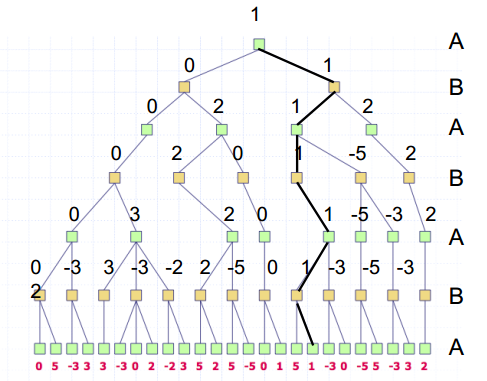
\includegraphics[width=0.6\linewidth]{fig/game-tree.png}
\end{figure}

用DFS可以遍历整棵树,同时保持线性的空间复杂度,每次回溯时更新结点为min/max即可

\subsubsection{Alpha-Beta剪枝}
注意$\alpha$-$\beta$剪枝只要有一祖先大于/小于后代节点的值就可以进行剪枝,即要看\textemph{所有祖先做决定}。
\begin{itemize}
	\item 只要当前Max结点的值$\geq$祖先某一Min结点的值,就可以在该Max结点上做$\alpha$剪枝
	\item 只要当前Min结点的值$\leq$祖先某一Max结点的值,就可以在该Min结点上做$\beta$剪枝
\end{itemize}
即\textemph{当前Min小等祖先Max,当前Max大等祖先Min可剪枝}。
\begin{algorithm}[H]
\caption{Alpha-Beta Pruning}
\begin{algorithmic}[1]
\Procedure{AlphaBeta}{n,Player,alpha,beta}
\If{n is TERMINAL}
\State \Return V(n)\Comment{Return terminal states utility}
\EndIf
\State ChildList = n.Successors(Player)
\If{Player == MAX}
\For{c in ChildList}
\State alpha = max(alpha, AlphaBeta(c,MIN,alpha,beta))
\If{beta $<=$ alpha}
\State break
\EndIf
\EndFor
\State \Return alpha
\Else\Comment{Player == MIN}
\For{c in ChildList}
\State beta = min(beta, AlphaBeta(c,MAX,alpha,beta))
\If{alpha $>=$ beta}
\State break
\EndIf
\EndFor
\State \Return beta
\EndIf
\EndProcedure\Comment{Initial call: AlphaBeta(START-NODE,Player,$-\infty$,$+\infty$)}
\end{algorithmic}
\end{algorithm}

\begin{example}
如下采用$\alpha-\beta$剪枝进行搜索,方形为Max结点,圆形为Min结点。
\begin{figure}[H]
\centering
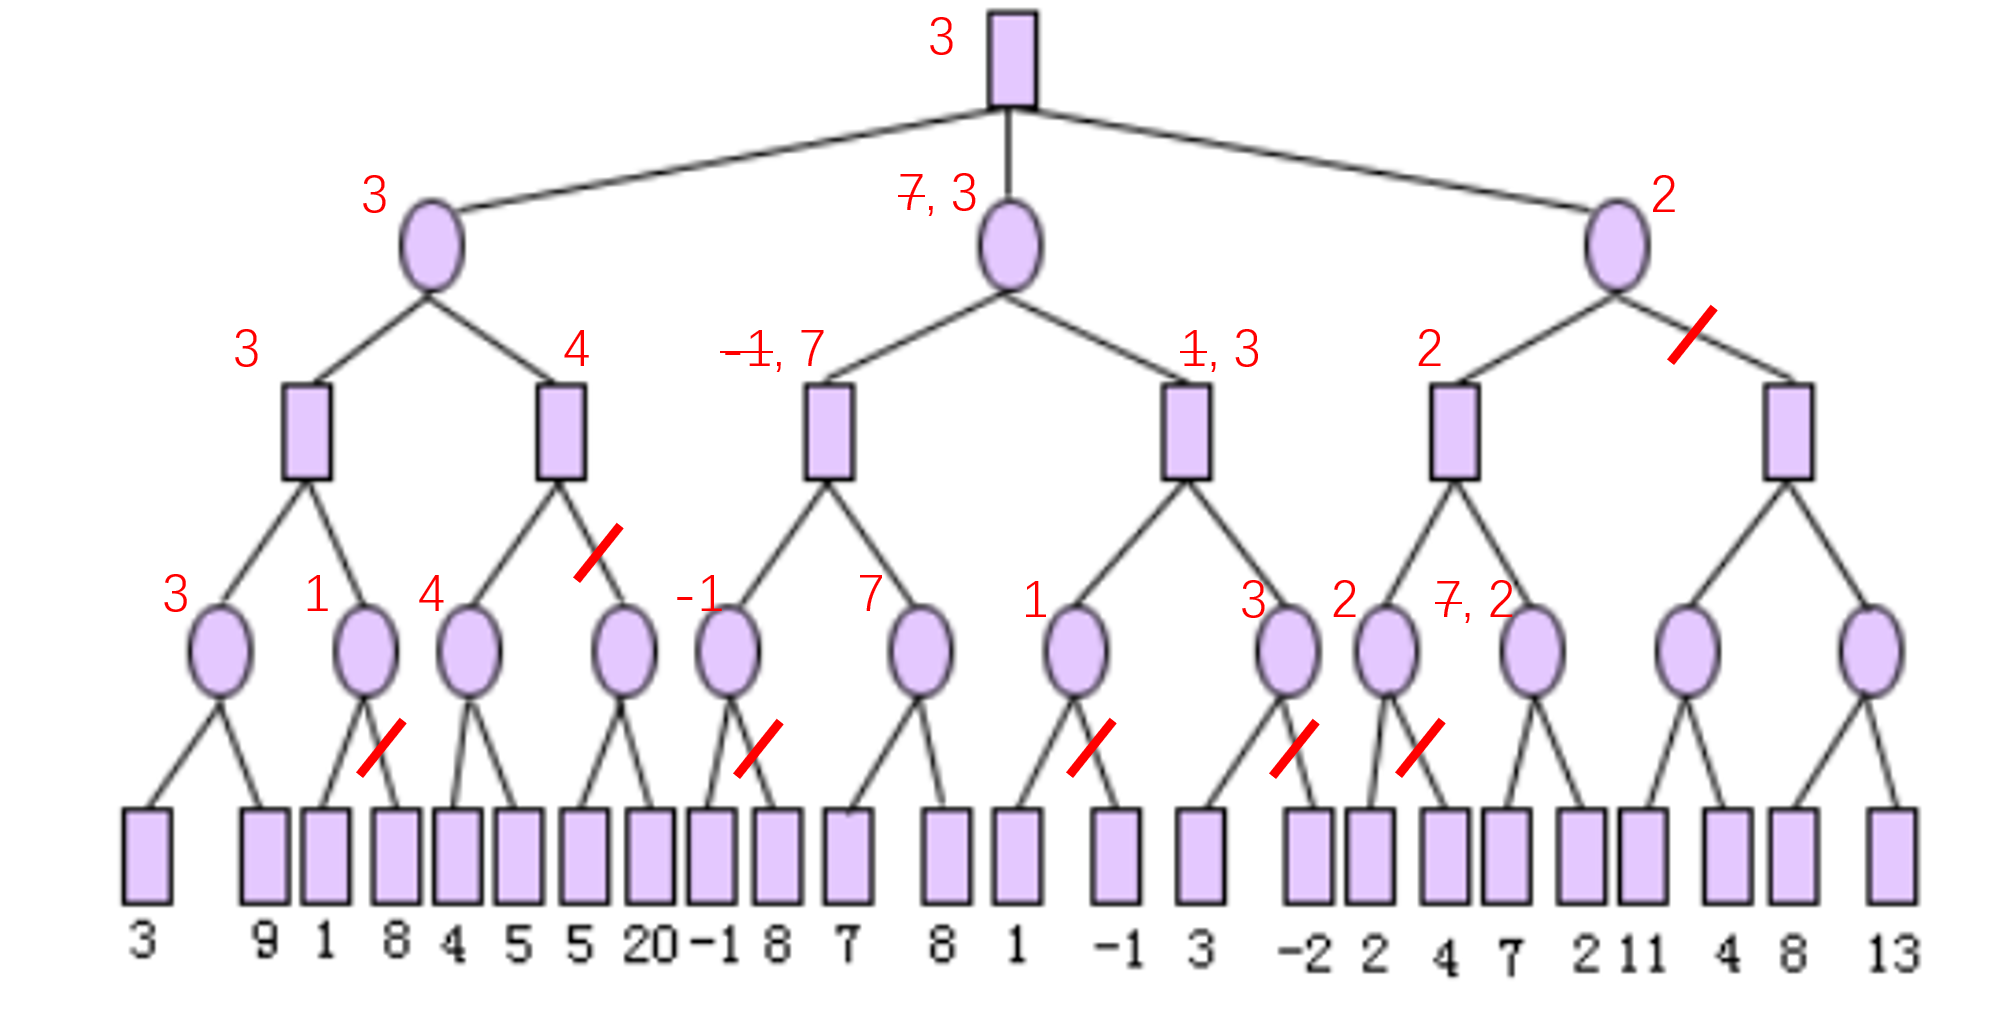
\includegraphics[width=0.9\linewidth]{fig/T01-3.png}
\end{figure}
\end{example}

可以证明,如果原始情况需要访问$O(b^D)$个结点,则经过$\alpha$-$\beta$剪枝后只需访问$O(b^{D/2})$个结点。

\subsubsection{其他补充}
但在现实生活的游戏中,即使采用了$\alpha$-$\beta$剪枝,博弈树也太过庞大。
如棋类的分支因子大致是35,深度为10的树已经到$2.7\times 10^{14}$个结点。
因此不能将整棵博弈树展开,需要采用一些启发式方式进行估计。

评价函数(evaluation)的一些需求:
\begin{itemize}
	\item 对于终止状态,评价函数的序应与真实的收益函数相同
	\item 对于非终止状态,评价函数则应该与真实的胜率相关联
	\item 计算时间不能花太长
	\item 通常取多个特征,然后进行加权求和(先验知识)
\end{itemize}

在线(online)/实时(real-time)搜索
\begin{itemize}
	\item 没有办法展开全部的边界集,因此限制展开的大小(在没找到去目标的真实路径就做出决定/直接选一条路就开始走)
	\item 在这种情况下,评价函数不仅仅引导搜索,更是提交真实的动作
	\item 虽然找不到最优解,但是求解时间大大缩减
\end{itemize}
% !TEX root = main.tex

\section{限制可满足性问题}
% CSP: Formalization, backtracking, forward checking, and GAC algorithms

在搜索问题中,状态表示是个黑箱,可以有多种多样的方法来表达。
但实际上我们可以有特定的状态表示方法来解决大量不同的问题,在这种情况下的搜索算法可以变得很高效。

限制可满足性问题(Constraint Satisfaction Problem, CSP)指每一个状态都可以用一组特征值向量表示的问题。
\begin{itemize}
	\item $k$个特征/\textemph{变量}的集合$V_1,\ldots,V_n$
	\item 每一个变量都有一个包含有限值的\textemph{论域}$\dom[V_i]$,如
	\[\text{height}=\{\text{short},\text{average},\text{tall}\}\]
	\item 一组\textemph{限制条件}$C_1,\ldots,C_m$
	\begin{itemize}
		\item 每个限制条件都有一个作用域(scope),表示作用在什么变量上,如$C(V_1,V_2,V_4)$
		\item 相当于一个布尔函数,从变量赋值到布尔值的映射,如
		\[C(V_1=a,V_2=b,V_4=c)=True\]
		\item 布尔函数可以以表形式给出,或以表达式形式给出,如$C(V_1,V_2,V_4)=(V_1=V_2+V_4)$
		\item \textemph{注意限制是否写了变量不同allDifferent(Vars)},这一条在很多问题中都会出现
	\end{itemize}
	\item 一个状态可以通过给每一个变量赋值得到
\end{itemize}

CSP不关心到目标状态的移动步骤,而只关心是否存在这样一组变量满足目标。

\subsection{回溯搜索(Backtracking)}
对每一个变量分别赋值,深搜方式,同时结合启发式函数,用于在每一步选择不同的赋值变量。
\begin{figure}[H]
\centering
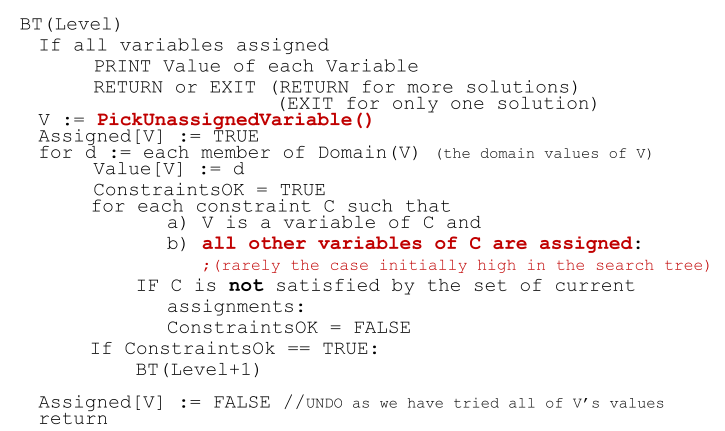
\includegraphics[width=0.6\linewidth]{fig/backtracking.png}
\end{figure}
\begin{figure}[H]
\centering
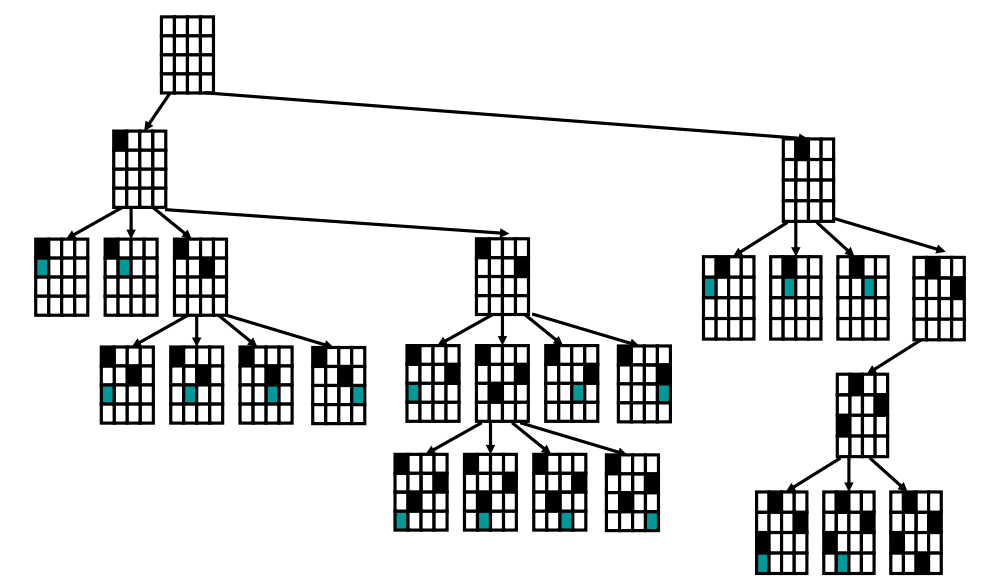
\includegraphics[width=0.6\linewidth]{fig/backtracking_eg.png}
\end{figure}

回溯的问题在于不能提前探测到某一变量已经没有可以赋值了,导致依然要进入一层进行搜索。
因此考虑前瞻式算法,即限制传播(propagation)。
\begin{itemize}
	\item 甚至可以在还未进行搜索之前就采用
	\item 传播本身需要耗费资源,因此这里存在一个权衡
\end{itemize}
进而有下列两种传播算法:前向传播和GAC算法。

\subsection{向前检测(Forward Checking)}
\begin{enumerate}
	\item 选择一个未被赋值的变量$V$。这里可以采用\textbf{最小剩余值}(Minimum Remaining Values, MRV)作为启发式函数,即先选论域小的变量。
	\item 选择论域$\dom[V]$中的值对$V$进行赋值$d$
	\item 将$d$向前传递给含有$V$的限制$C$,主要考察那些\textbf{只剩一个未赋值变量$X$}的限制
	\item 检测\verb'FCCheck(C,X)'是否出现论域清空(Domain Wipe Out, DWO),即$X$没得选值了。
	这里\verb'FCCheck'做的则是核心的限制传播部分,当$V=d$后把$X$不能取的值删去
	\item 如果不出现DWO,则进入下一层(选择新的未赋值变量赋值)
	\item 否则需要恢复当层\verb'FCCheck'剪枝的部分,即\textemph{$d$不可取(注意这里移除的是原变量$V$中的值)},$V$要重新取值
\end{enumerate}
\begin{figure}[H]
\centering
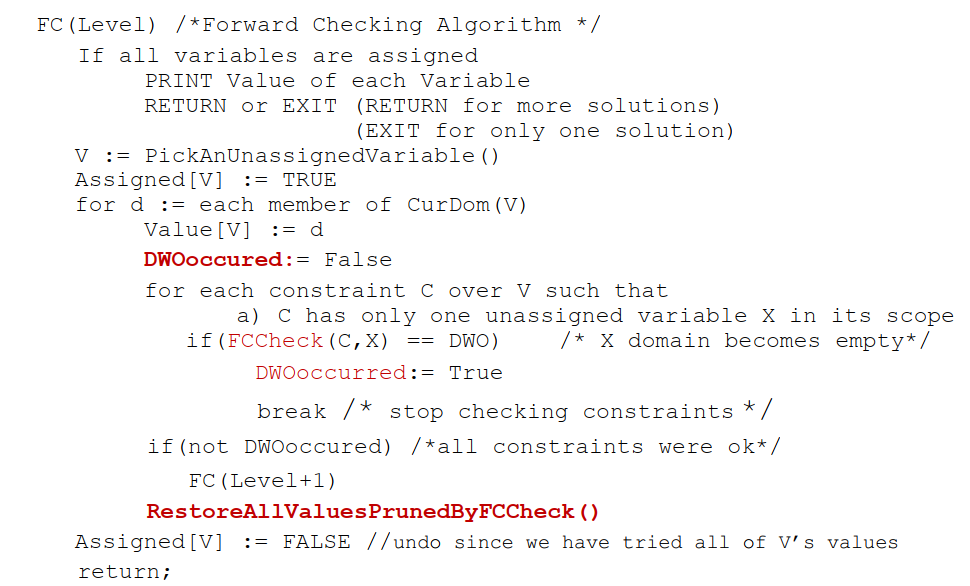
\includegraphics[width=0.6\linewidth]{fig/forward_checking.png}
\end{figure}
\begin{figure}[H]
\centering
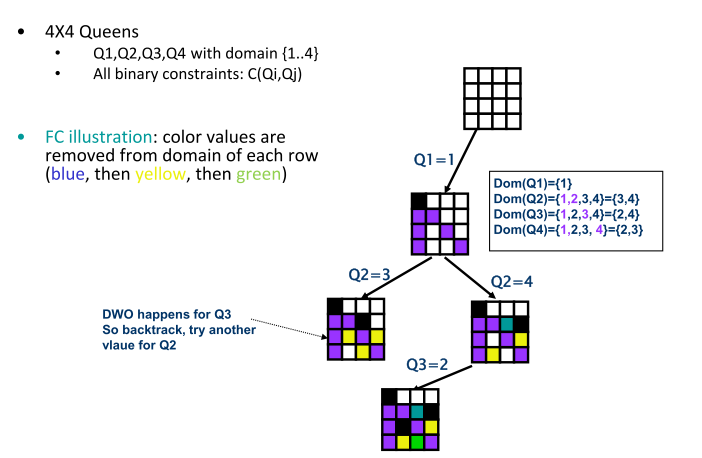
\includegraphics[width=0.6\linewidth]{fig/forward_checking_eg.png}
\end{figure}

其实这是人工解数独一种很常见的方法,即当前格填了某一个值后会不会导致其他格填不了,可以进行试探然后将其他格中不能填的值都去除(约束传播)。

\subsection{泛化边一致性(GAC)}
\begin{definition}[一致]
限制$C(X,Y)$是一致的,当且仅当对于所有$X$的值都存在某些$Y$满足$C$,即$\forall X\exists Y:C(X,Y)$。
\end{definition}
\begin{definition}[泛化边一致性(Generalized Arc Consistency, GAC)]
限制$C(V_1,V_2,\ldots,V_n)$是关于$V_i$边一致的,当且仅当$\forall V_i,\exists V_1,\ldots,V_{i-1},V_{i+1},\ldots,V_n$满足$C$。
限制$C$是GAC的当且仅当对于每一变量都是GAC的。
一个CSP是GAC的当且仅当它的限制都是GAC的。
\end{definition}

有GAC算法:
\begin{itemize}
\item 在$V_i=d$下,没有其他变量赋值能够满足该限制,则$d$是边不一致的,进而$V_i=d$可以被剪枝剪掉。
\item 注意当从论域中移除一个值时可能导致新的不一致,故需要采用队列的方式,不断将需要检测边一致性限制添加(即\textemph{包含被移除值变量$V$的限制}),直到队列为空,即限制条件变为GAC。
\item 近似可理解为将后续搜索步骤都前移到剪枝部分。
\item 注意在未进入循环之前就可以先进行检测了。
\end{itemize}
\begin{figure}[H]
\centering
\begin{tabular}{cc}
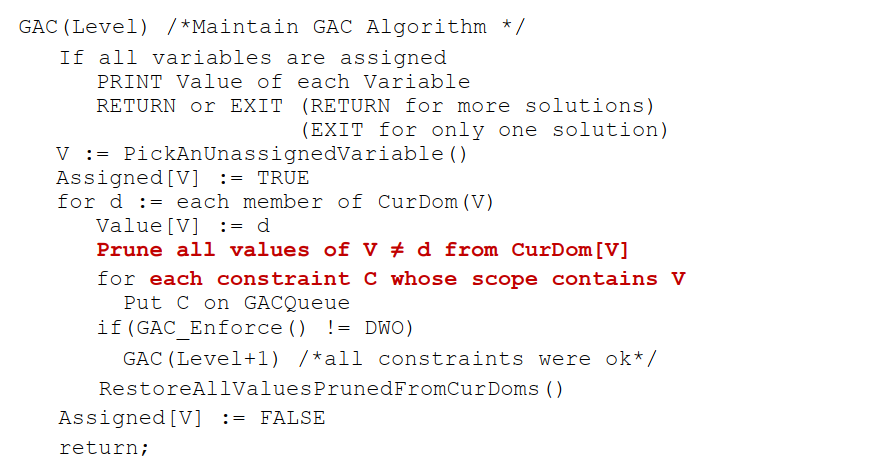
\includegraphics[width=0.5\linewidth]{fig/gac.png}&
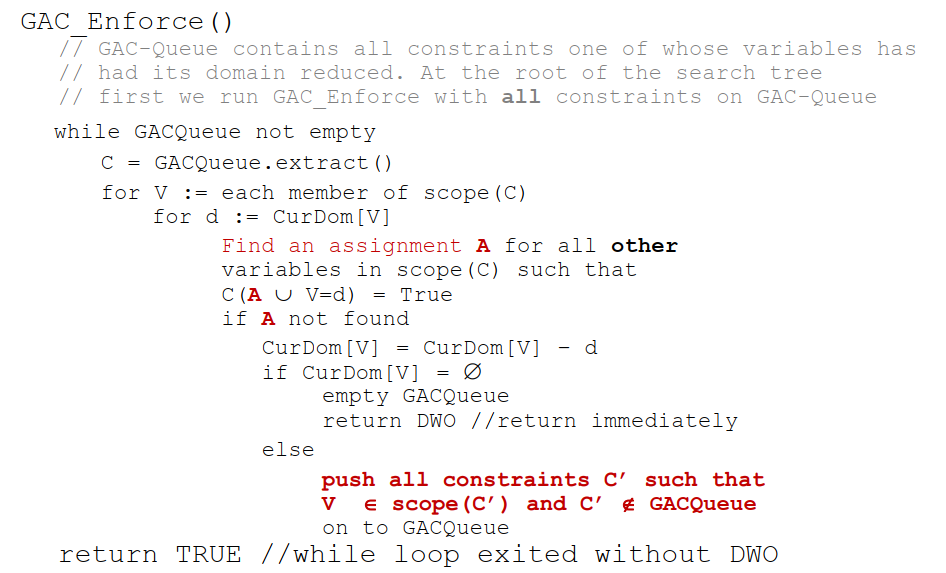
\includegraphics[width=0.5\linewidth]{fig/gac_enforce.png}
\end{tabular}
\end{figure}
\begin{figure}[H]
\centering
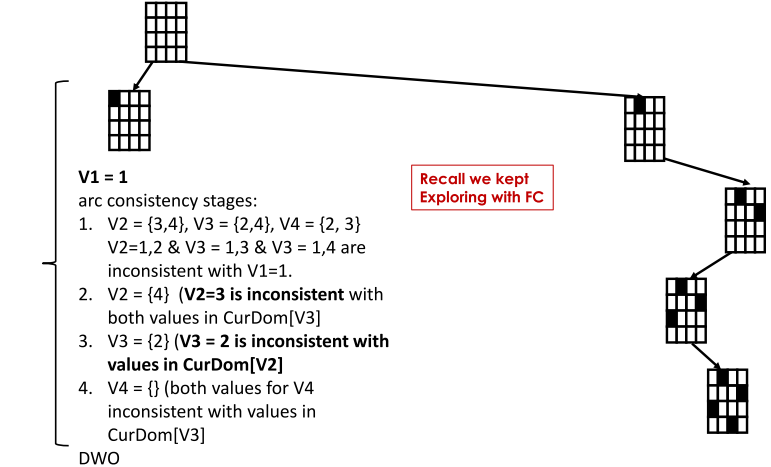
\includegraphics[width=0.6\linewidth]{fig/gac_eg.png}
\end{figure}

其实如果直接手跑实验,则同样类比数独,先将每一个格不能填的数字都划掉(循环添加条件直至收敛),然后尝试赋值进入下一层。
\begin{example}
考虑$5$个变量$A,B,C,D,E$,论域都为$\{1,2,3,4\}$,限制条件为$A > D$,$D > E$,$C \ne A$,$C > E$,$C \ne D$,$B \geq A$,$B \ne C$和$C \ne D + 1$。
\end{example}
\begin{analysis}
\begin{figure}[H]
\centering
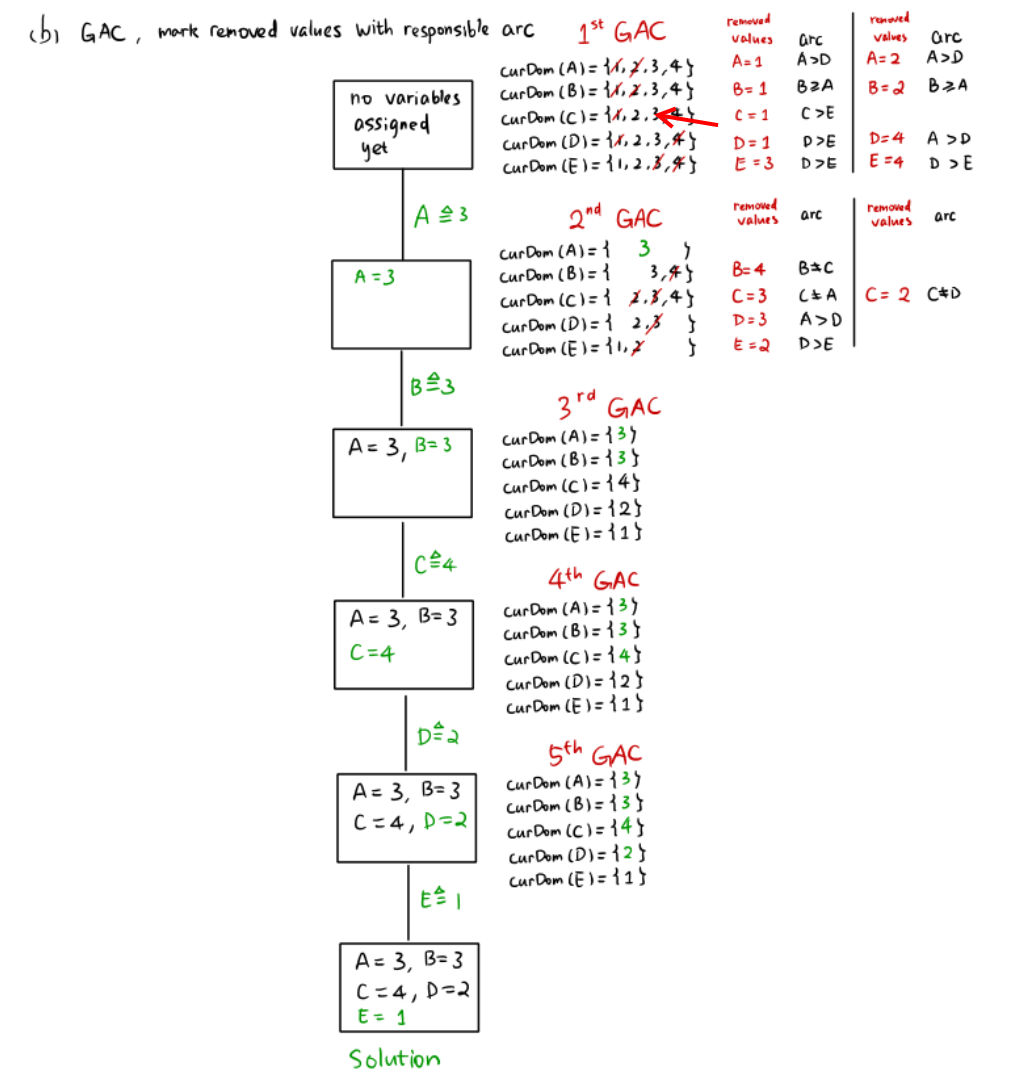
\includegraphics[width=0.7\linewidth]{fig/T02-2.png}
\end{figure}
\end{analysis}

\begin{definition}[支撑]
在限制$C$下变量赋值$V=d$的支撑是对$C$中其他变量的赋值$A$,使得$A\cup\{V=d\}$满足$C$。
即\textemph{其他变量的指派构成了当前变量的支撑}。
\end{definition}

向前检测和边一致性检测的区别如下,即FC只考虑当前限制下某一变量赋值带来的后果,而GAC则考虑所有限制下变量赋值带来的后果。
\begin{figure}[H]
\centering
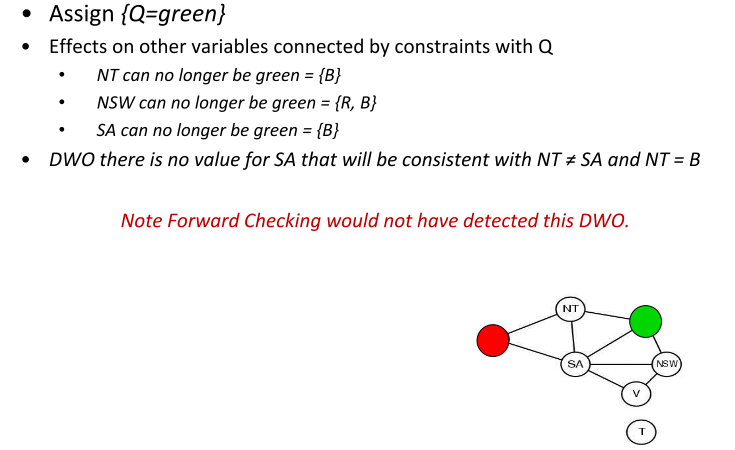
\includegraphics[width=0.8\linewidth]{fig/diff_fc_gac.png}
\end{figure}
% !TEX root = main.tex

\section{知识表示与推理}
\subsection{基本概念}
一阶逻辑(First-Order Logic,FOL)
\begin{itemize}
	\item 个体/常量(0-arity)
	\item 一元(unary)谓词:$A(x),B(x)$
	\item 关系/二元谓词:$L(x,y)$
\end{itemize}

\begin{definition}[项(term)]
每一个变量都是一个项。
若$t_1,\ldots,t_n$都为项,且$f$为$n$参数的的函数符号,则$f(t_1,\ldots,t_n)$是一个项。
\end{definition}
\begin{definition}[公式(formular)]
公式包括以下几种情况:
\begin{itemize}
\item 若$t_1,\ldots,t_n$都是项,且$P$是$n$元的谓词符号,则$P(t_1,\ldots,t_n)$是一个公式
\item 若$t_1,t_2$都是项,那么$(t_1=t_2)$是一个原子公式
\item 若$\alpha,\beta$都是公式,$v$是一个变量,则$\lnot\alpha,(\alpha\land\beta),(\alpha\lnot\beta),\exists v.\alpha,\forall v.\alpha$都是公式
\end{itemize}
注意公式中的变量是自由的(free)还是约束的(bound),通过全称特称符号可进行约束。
没有自由变量的公式称为句子(sentence)。
\end{definition}
\begin{definition}[替换]
$\alpha[v/t]$表示$\alpha$中所有自由出现的$v$都用项$t$替代
\end{definition}
\begin{definition}[解释(interpretation)]
一个解释是一个对(pair)$\mI=\lrang{D,I}$,其中
\begin{itemize}
	\item $D$是论域,可以是任何非空集
	\item $I$是从谓词到函数符号的映射
	\item 若$P$是一个$n$元谓词符号,则$I(P)$是一个在$D$上的$n$元关系,即$I(P)\subset D^n$。
	如$p$是一个常量/命题符号,则$I(p)\in\{True,False\}$。
	\item 若$f$是一个$n$元函数符号,则$I(f)$是一个在$D$上的$n$元函数,即$I(f):D^n\to D$。
	如$c$是一个零元常量符号,则$I(c)\in D$。
\end{itemize}
\end{definition}
\begin{definition}[赋值(denotation)]
变量指派(assignment)$\mu$是一个从变量集合到论域$D$的映射
\[\begin{aligned}
\norm{v}_{\mI,\mu}&=\mu(v)\\
\norm{f(t_1,\ldots,t_n)}_{\mI,\mu}&=I(f)(\norm{t_1}_{\mI,\mu},\ldots,\norm{t_n}_{\mI,\mu})
\end{aligned}\]
\end{definition}
\begin{definition}[满足]
$\mI,\mu\models\alpha$读作$\mI,\mu$满足$\alpha$
\begin{itemize}
	\item $\mI,\mu\models P(t_1,\ldots,t_n)\iff\lrang{\norm{t_1}_{\mI,\mu},\ldots,\norm{t_n}_{\mI,\mu}}\in I(P)$
	\item $\mI,\mu\models(t_1=t_2)\iff\norm{t_1}_{\mI,\mu}=\norm{t_2}_{\mI,\mu}$
\end{itemize}
同样也有命题逻辑的一些性质
\begin{itemize}
	\item $\mI,\mu\models\lnot\alpha\iff\mI,\mu\not\models\alpha$
	\item $\mI,\mu\models(\alpha\land\beta)\iff(\mI,\mu\models\alpha\land\mI,\mu\models\beta)$
	\item $\mI,\mu\models(\alpha\lor\beta)\iff(\mI,\mu\models\alpha\lor\mI,\mu\models\beta)$
	\item $\mI,\mu\models\exists v.\alpha\iff(\exists d\in D:\mI,\mu\{d;v\}\models\alpha)$
	\item $\mI,\mu\models\forall v.\alpha\iff(\forall d\in D:\mI,\mu\{d;v\}\models\alpha)$
\end{itemize}

令$S$为句子的集合,若对于所有$\alpha\in\mI,\mI\models\alpha$,则称$\mI$满足$S$,记作$\mI\models S$,$\mI$又被称为$S$的一个模型。
若$S$是可满足的,则存在$\mI$使得$\mI\models S$。
\end{definition}
\begin{example}
通常的问题是下列句子集合是否是可满足的
\[\{\forall x(P(x)\to Q(x)),P(a),\lnot Q(a)\}\]
即是否存在这样的解释/变量赋值使全部句子都成立。
\end{example}

\begin{definition}[蕴含(entail)]
$S\models\alpha$是指对于任意满足$\mI\models S$的$\mI$有$\mI\models\alpha$,读作$S$蕴含$\alpha$或$\alpha$是$S$一个逻辑结果(consequence)。
注意$\{\alpha_1,\ldots,\alpha_n\}\models\alpha$当且仅当$\alpha_1\land\cdots\land\alpha_n\to\alpha$合法,当且仅当$\alpha_1\land\cdots\land\lnot\alpha$不可满足。
\end{definition}
\begin{example}
令知识库$KB$为句子集合,$\alpha$为一个询问,想要知道知识库是否能推出询问,即求蕴含$KB\models\alpha$。
若要证明$KB\not\models\alpha$,则只需给出一个解释满足$KB$但不满足$\alpha$。
\end{example}

\subsection{推理}
\subsubsection{归结}
\begin{definition}[子句(clause)]
文字(literal)是原子公式或它的取反,一个子句是文字的析取(disjunction),如$p\lor\lnot r\lor s$,写作$(p,\lnot r,s)$。
特殊地,空子句$()$代表为假。
公式(formula)则是子句的合取(conjunction)。
\end{definition}

\begin{definition}[归结(resolution)]
从两条子句$\{p\}\cup c_1$和$\{\lnot p\}\cup c_2$中推出子句$c_1\cup c_2$的过程称为归结。
\end{definition}
\begin{definition}[获取(derivation)]
句子序列$c_1,\ldots,c_n=c$,对于每一个$c_i$,或者$c_i\in S$,或者$c_i$是先前\textemph{两个子句}的归结,这个过程称为获取,记为$S\vdash c$。
\end{definition}
\begin{theorem}
若$S\vdash c$,则$S\models c$
\end{theorem}
但注意其逆命题并不成立,考虑$(p)\models(p,q)$,但是$(p)\nvDash(p,q)$。

\begin{theorem}
$S\vdash()\iff S\models()\iff S$是不可满足的
\end{theorem}

进而得到基于归结的推理过程:反驳(refutation),即$KB\models\alpha\iff KB\land\alpha$是不可满足的
\begin{itemize}
	\item 将$KB$和$\lnot\alpha$改写为子句形式构成$S$
	\item 检测是否$S\vdash()$
\end{itemize}
\begin{figure}[H]
\centering
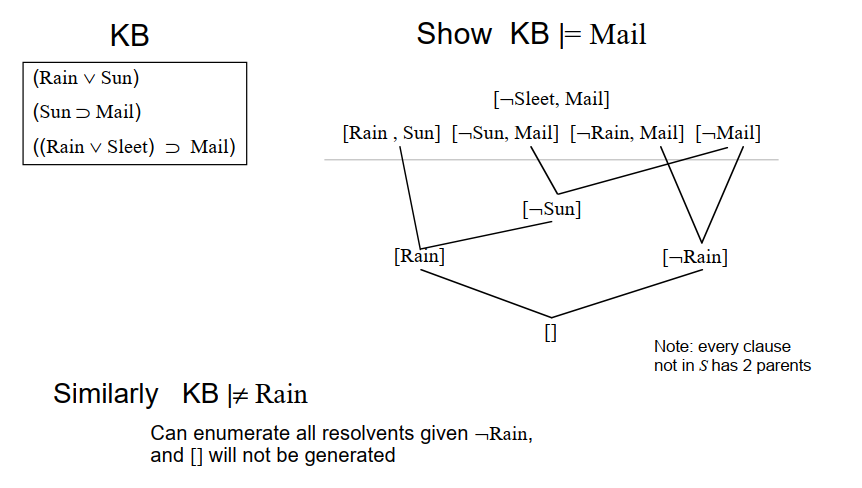
\includegraphics[width=0.8\linewidth]{fig/refutation.png}
\end{figure}

利用归结(两条文字合一变真删除)看是否能得到空子句。

\subsubsection{子句形式转换}
\begin{itemize}
	\item 消除蕴含:$A\to B\iff \lnot A\lor B$
	\item 将非向内推:德摩根定律
	\item 标准化变量:重命名变量使得每一个量词都是唯一的
	\item 消除存在量词(skloemize):引入新的函数符号,如$\forall x P(x)$改为$P(g(y))$
	\item 将所有量词带到最前面:只有全局量词,且名字均不同
	\item 析取分配到合取
	\item 压平嵌套合取和析取
	\item 转化为子句:将量词全部移除,然后分离成几条子句
\end{itemize}

\subsubsection{合一}
归结过程中可能需要合一(unification),用来消除两个子句中不同的变量。
\begin{definition}[合一子(unifier)]
令公式$f$和$g$语义等价的替换$\sigma$称为$f$和$g$的合一子
\end{definition}
\begin{example}
$P(f(x),a)$和$P(y,f(w))$不能被合一,因没有令$a=f(w)$的替换使得两者相同
\end{example}

\begin{definition}[最一般合一子(Most General Unifier, MGU)]
两个公式$f$和$g$的替换$\sigma$是MGU,若
\begin{itemize}
	\item $\sigma$是一个合一子
	\item 对于其他合一子$\theta$必然存在第三个替换$\lambda$使得$\theta=\sigma\lambda$
\end{itemize}
也就是说其他的合一子都比$\sigma$更特殊(specialized)。
\end{definition}
\begin{example}
考虑$P(f(x),z)$和$P(y,a)$
\begin{itemize}
	\item $\sigma=\{y=f(a),x=a,z=a\}$是一个合一子,但不是MGU
	\item $\theta=\{y=f(x),z=a\}$是一个MGU
	\item $\sigma=\theta\lambda$,其中$\lambda=\{x=a\}$
\end{itemize}
\end{example}

计算MGU的算法:不断代入新的元,使其一致
\begin{figure}[H]
\centering
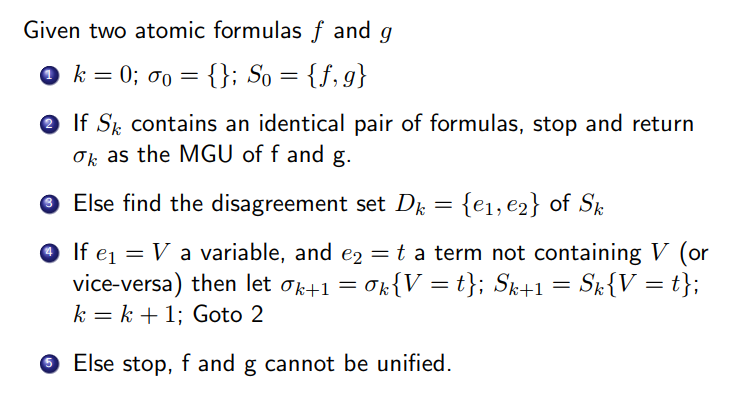
\includegraphics[width=0.8\linewidth]{fig/MGU.png}
\end{figure}

\subsubsection{完整例子}
\textbf{基于反驳的归结推理}
\begin{figure}[H]
\centering
\begin{tabular}{c}
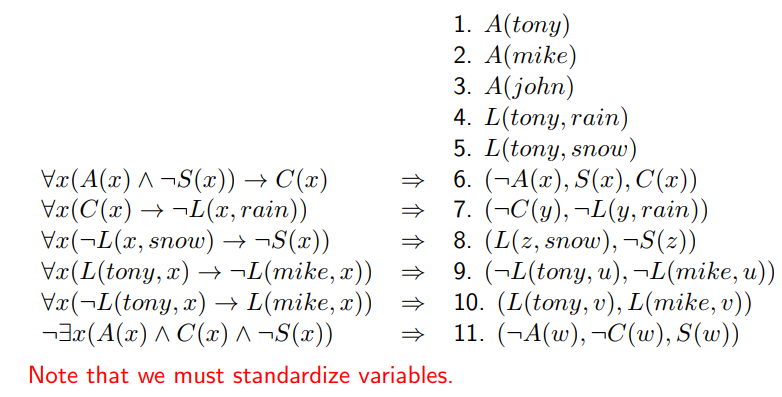
\includegraphics[width=0.8\linewidth]{fig/alpine_club_eg1.png}\\
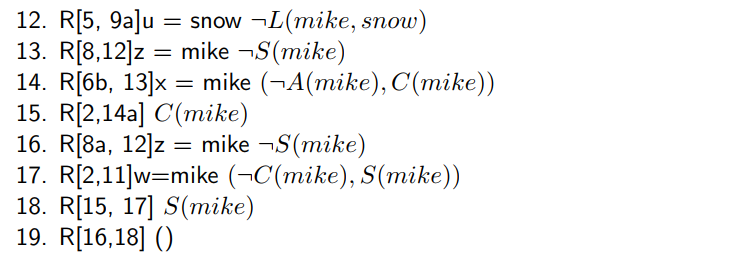
\includegraphics[width=0.8\linewidth]{fig/alpine_club_eg2.png}
\end{tabular}
\end{figure}

\myhline
\textbf{答案抽取(answer extraction)}
\begin{itemize}
\item 将询问$\exists xP(x)$用$\exists x[P(x)\land\lnot\text{answer}(x)]$替换
(因为取非后变成$\forall x P(x)\implies \text{answer}(x)$)
\item 直到获得任意子句只包含答案的谓词
\end{itemize}
\begin{example}
对下列查询进行归结及答案查询
\begin{itemize}
	\item Whoever can read $R(x)$ is literate $L(x)$
	\item Dolphins $D(x)$ are not literate
	\item Flipper is an intelligent dolphin $I(x)$
\end{itemize}
Who is intelligent but cannot read?
\end{example}
\begin{analysis}
对语句进行形式化
\begin{center}
\begin{tabular}{lll}
$\forall x (R(x)\to L(x))$ & 1 & $(\lnot R(u),L(u))$\\
$\forall x (D(x)\to \lnot L(x))$ & 2 & $(\lnot D(v),\lnot L(v))$\\
$D(Flip)\land I(Flip)$ & 3 & $D(Flip)$\\
 & 4 & $I(Flip)$\\
Q:$\exists x (I(x)\land\lnot R(x))$ & 5 & $(\lnot I(y),R(y),answer(y))$\\\hline 
$R[4,5]/y=Flip$ & 6 & $(R(Flip),answer(Flip))$\\
$R[1,6]/u=Flip$ & 7 & $(L(Flip),answer(Flip))$\\
$R[2,7]/v=Flip$ & 8 & $(\lnot D(Flip),answer(Flip))$\\
$R[3,8]$ & 9 & $(answer(Flip))$
\end{tabular}
\end{center}
因此得到Flipper是聪明的但是不能阅读
\end{analysis}
% !TEX root = main.tex

\section{确定性规划}
智能体应该能够对世界做出动作(action),而不仅仅是通过搜索解决问题或推理及知识表示。
核心是对动作的效果进行推理,并且计算什么动作能够达成特定的效果。

本节中主要关注确定性规划,即有完全的初始状态描述及确定性的动作效果。

\subsection{情景演算}
情景演算(Situation Calculation, SitCalc)三个基本部分
\begin{itemize}
	\item 动作(action):一组谓词
	\item 情景(situations):动作序列,$do(a,s)$为动作、情景到新情景的函数映射,$S_0$为初始情景
	\[do(put(a,b),do(put(b,c),S_0))\]
	要区别情景与状态(state),如将硬币转两次,情景/动作历史不同,但状态都是一样的
	\item 流(fluent):从情景到情景的谓词或函数(动态变化过程),用谓词或函数符号描述,其中最后一个参数为情景,如$Holding(r,x,s)$代表机器人$r$在状态$s$下拿着物体$x$,有
	\[\lnot Holding(r,x,s)\land Holding(r,x,do(pickup(r,x),s))\]
	\item 条件(precondition):动作执行的前提条件
	\item 影响(effect):执行动作后改变的流。 % the fluents that change as the result of performing the action
	如下在情景$s$下执行修复动作后,$x$就不是破碎的
	\[\lnot Broken(x,do(repair(r,x)),s)\]
\end{itemize}

情景演算的形式化仅陈述了执行动作的影响,而没有阐述没影响的部分。
但是给定一个流只有很少的动作会被影响,而大多数都保持不变。

而框架(frame)问题则是找到一种高效的方法来确定动作的非效果(non-effects)。而不是显式地将它们全部写下来,可以考虑用一阶逻辑。

形式化后的情景即可以利用归结进行规划,但是开销会非常大。

\subsection{STRIPS}
传统的规划没有不完全或不确定的信息,因此可以做以下假设。
\begin{itemize}
	\item 封闭世界假设(Closed-World Assumption, CWA):初始状态的信息是完备的,用于表示世界状态的知识库是一系列真实的原子事实(与数据库类似)。
	如$emp(A,C)$不在数据库中,则$\lnot emp(A,C)$为真。
	\item 动作的前提只能是原子命题的合取
	\item 动作的影响只会使原子命题变真或变假,不会出现条件影响或析取影响
\end{itemize}

STRIPS(Stanford Research Institute Problem Solver):
\begin{itemize}
	\item 世界被表示成封建世界知识库(CW-KB),一个STRIPS的动作表示成更新CW-KB的方式
	\item 一个动作生成新的KB,用以描述新的世界
\end{itemize}

在SitCalc中我们可能有不完全的信息(用一阶逻辑公式表示),而在STRIPS中,我们有完整的信息(用CW-KB)表示。

STRIPS中需要用3个列表来表示一个动作
\begin{itemize}
	\item 动作的前提\verb'pre'
	\item 动作增加的影响\verb'add'
	\item 动作减少的影响\verb'delete'
\end{itemize}

例子如下:
$pickup(X)$:
\begin{itemize}
\item $Pre: {handempty, clear(X), ontable(X)}$
\item $Adds: {holding(X)}$
\item $Dels: {handempty, clear(X), ontable(X)}$
\end{itemize}

\myhline
注意STRIPS的表达力还是有限制的,如它没有条件(conditional)影响。
因此需要有表达力更强的语言Action Description Language(ADL),允许在前提中有任意公式,而且可以有条件和全称影响。

可以将规划看成是一个搜索问题,每个动作都是由一个CW-KB到CW-KB的映射,但搜索空间会非常巨大。

\subsection{松弛问题}
放松(relaxed)问题即考虑\textbf{忽略删除动作}的列表,这样可能得到有用的启发式函数估计。

\begin{theorem}
放松问题的一个最优规划的长度是原始问题最优规划长度的下界
\end{theorem}
\begin{proof}
由于我们将所有影响都添加了,并且不删除负面影响,因此很直觉地会很快得到目标。
令$P$为原始问题,$P'$为放松问题,我们希望得到$Sols(P)\subset Sols(P')$,则有$Minlen(Sols(P'))\leq Minlen(Sols(P))$。
\begin{itemize}
\item 令$a_0,\ldots,a_{n-1}$为$P$的解,证明它也是$P'$的一个解。
令$s_0$为初始状态,令$s_{i+1}=s_i\cup add(a_i)-del(a_i),\forall i<n$,且$Goal\subset s_n$,$pre(a_i)\subset s_i,\forall i < n$。
\item 又令$s_0'=s_0$,且$s_{i+1}'=s_i'\cup add(a_i)$,通过数学归纳法证明$s_i\subset s_i',\forall i \leq n$。
\begin{itemize}
	\item 归纳奠基:$i=0$时$s_0\subset s_0'=s_0$
	\item 归纳假设:假设$s_i\subset s_i',\forall i<n$,证明$s_{i+1}\subset s_{i+1}'$
	\item 推理:因为$a_i$在$s_i$中是可采纳的,即$pre(a_i)\subset s_i$,因此$pre(a_i)\subset s_i\subset s_i'$,即$a_i$在$s_i'$中是可采纳的。所以得到
	\[s_{i+1}=s_i\cup add(a_i)-del(a_i)\subset s_i'\cup add(a_i)=s_{i+1}'\]
\end{itemize}
\end{itemize}
进而$Goal\subset s_n\subset s_n'$,且$pre(a_i)\subset s_i\subset s_i',\forall i<n$,因此$a_0,\ldots,a_{n-1}$也是$P'$的一个解。
\end{proof}

因此最优放松问题的规划可以作为$A^\star$算法的可采纳启发式函数。
然而在放松问题中计算一个最优的问题是NP难的,可以从$S$开始建立层次(layered)结构使其到达目标。

可达性分析:$s_0,a_1,s_1,\ldots,a_n,s_n$,直到$s_n\subset Goal$,或者状态层$s_n$不再改变(到达不动点)。
\begin{proposition}
令$a_0,\ldots,a_{n-1}$为$S_0$中可采纳的动作序列,令$s_0=S_0$,且$s_{i+1}=s_i\cup add(a_i)-del(a_i)$。
那么$\forall i<n,\exists j,k\leq i$使得$a_i\in A_k$且$s_i\subset S_j$
\end{proposition}
\begin{analysis}
用数学归纳法
\begin{itemize}
	\item 归纳奠基:$i=0$显然成立
	\item 归纳假设:假设$\forall i <n \exists j\leq i:\;s_i\subset S_j$
	\item 因为$pre(a_i)\subset s_i,pre(a_i)\subset S_j$,令$k$为最小的$u\leq j$使得$pre(a_i)\subset S_u$,那么$a_i\in A_k$,故$add(a_i)\subset S_{k+1}\subset S_{j+1}$
	因此
	\[s_{i+1}\subset s_i\cup add(a_i)\subset S_j\cup S_{j+1}=S_{j+1}\]
\end{itemize}
\end{analysis}

\begin{theorem}
假设$Goal\subset S_k$,对于$i<k$,令$A_{i-1}'$为调用CountActions($G_i,S_i$)的结果,则$A_0',\ldots,A_{k-1}'$为松弛问题的一个解。
\end{theorem}
\begin{proof}
用数学归纳法
\end{proof}

\begin{theorem}
假设状态层不再改变且目标不被满足,则原始规划问题是不可解的。
\end{theorem}
\begin{proof}
用反证法,假设$a_0,\ldots,a_{n-1}$为原始问题的一个解,则$Goal\subset s_n$。
由前面的命题,存在$m\leq n$使得$Goal\subset s_n\subset S_m$,导致矛盾。
\end{proof}
% !TEX root = main.tex

\section{不确定性规划}
% Bayesian networks: graphs + tables, inference
% Variable elimination algorithm
% Use D-separation to determine independence

\subsection{基础知识}
一组变量$V_1,\ldots,V_n$以及其对应的有限域$\dom[V_i]$,很容易导致指数的计算复杂度。
\begin{theorem}[全概率公式]
$\{B\}_{i=1}^k$为全集$U$的一个划分,则
\[\begin{aligned}
\pr{A}&=\pr{A\cap B_1}+\cdots+\pr{A\cap B_k}\\
&=\pr{A\mid B_1}\pr{B_1}+\cdots+\pr{A\mid B_k}\pr{B_k}
\end{aligned}\]
\end{theorem}
\begin{theorem}[条件独立]
若
\[\pr{B\mid A\cap C}=\pr{B\mid A}\]
,则在给定$A$的情况下$B$条件独立于$C$($C$没有给$A$增加知识)。
若对于所有$x\in\dom[X],y\in\dom[Y],z\in\dom[Z]$,
\[\pr{X=x\land Y=y\mid Z=z}=\pr{X=x\mid Z=z}\pr{Y=y\mid Z=z}\]
则在给定$Z=z$下,$X=x$和$Y=y$条件独立。
\end{theorem}
\begin{proposition}[独立性性质]
\begin{itemize}
	\item 若$A$和$B$独立,则$\pr{A\cap B}=\pr{A}\cdot\pr{B}$
	\item 给定$A$,$B$和$C$条件独立,则
	\[\pr{B\cap C\mid A}=\pr{B\mid A}\pr{C\mid A}\]
\end{itemize}
\end{proposition}
\begin{theorem}[贝叶斯公式]
条件概率定义
\[\pr{X\mid Y}=\pr{XY}/\pr{Y}\implies \pr{XY}=\pr{X\mid Y}\pr{Y}\]
注意与贝叶斯公式区分
\[\pr{Y\mid X}=\frac{\pr{XY}}{\pr{X}}=\frac{\pr{X\mid Y}\pr{Y}}{\pr{X}}\]
\end{theorem}
\begin{theorem}[链式法则]
\[\pr{A_1\cap A_2\cap\cdots\cap A_n}=\pr{A_1\mid A_2\cap\cdots\cap A_n}\pr{A_2\mid A_3\cdots\cap A_n}\pr{A_{n-1}\mid A_n}\pr{A_n}\]
% P(123) = P(1|23)P(2|3)P(3) = P(123)/P(23) P(23)/P(3) P(3)
\end{theorem}

\subsection{贝叶斯网络}
\subsubsection{基础知识}
\begin{bayesian}
E \arrow[r] & C\arrow[r] & A \arrow[r] & B\arrow[r] & H
\end{bayesian}
有以下概率公式成立
\begin{itemize}
	\item $\pr{H\mid B,A,E,C}=\pr{H\mid B}$
	\item 由链式法则和独立性假设
	\[\begin{aligned}
		\pr{HBACE}&=\pr{H\mid BACE}\pr{B\mid ACE}\pr{A\mid CE}\pr{C\mid E}\pr{E}\\
		\pr{HBACE}&=\pr{H\mid B}\pr{B\mid A}\pr{A\mid C}\pr{C\mid E}\pr{E}
	\end{aligned}\]
	\item 通用公式
	\[\pr{X_1X_2\cdots X_n}=\pr{X_n\mid Par(X_n)}\cdots\pr{X_1\mid Par(X_1)}\]
	\item 单点概率(由全概率公式和条件概率定义)
	\[\begin{aligned}
		\pr{a}&=\sum_{c_i\in\dom[C]}\pr{a\mid c_i}\pr{c_i}\\
		&=\sum_{c_i\in\dom[C]}\pr{a\mid c_i}\sum_{e_i\in\dom[E]}\pr{c_i\mid e_i}\pr{e_i}
	\end{aligned}\]
\end{itemize}

因此每个结点只需存一个条件概率表(conditional probability table, CPT)。

\begin{definition}[D分隔(separation)]
若一组变量$E$阻隔(block)了$X$到$Y$的所有\textcolor{red}{无向路径}$P$,则称$E$ D-分隔了$X$和$Y$,且有给定证据$E$下,$X$和$Y$条件独立。
$E$阻隔(block)了路径$P$当且仅当在路径上存在某点$Z$使得下面任一成立。
\begin{figure}[H]
\centering
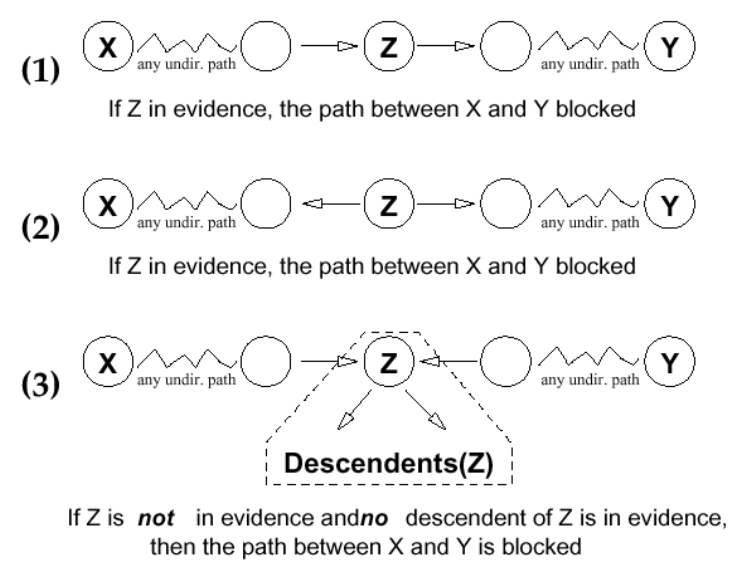
\includegraphics[width=0.8\linewidth]{fig/blocking.png}
\end{figure}
注意第3种情况,证据集中没有给交叉结点及其子结点,则父亲节点都独立。
\end{definition}
\begin{example}
考虑如下贝叶斯网络
\begin{bayesian}
A\arrow[dr] & & B\arrow[dl] \arrow[dr] & \\
 & C\arrow[dl] \arrow[dr] & & D\\
E & & F &
\end{bayesian}
在此例中$\pr{c\mid a,b,\lnot d,\lnot e,\lnot f}\ne\pr{c\mid a,b}$。
\end{example}
\begin{example}
\begin{figure}[H]
\centering
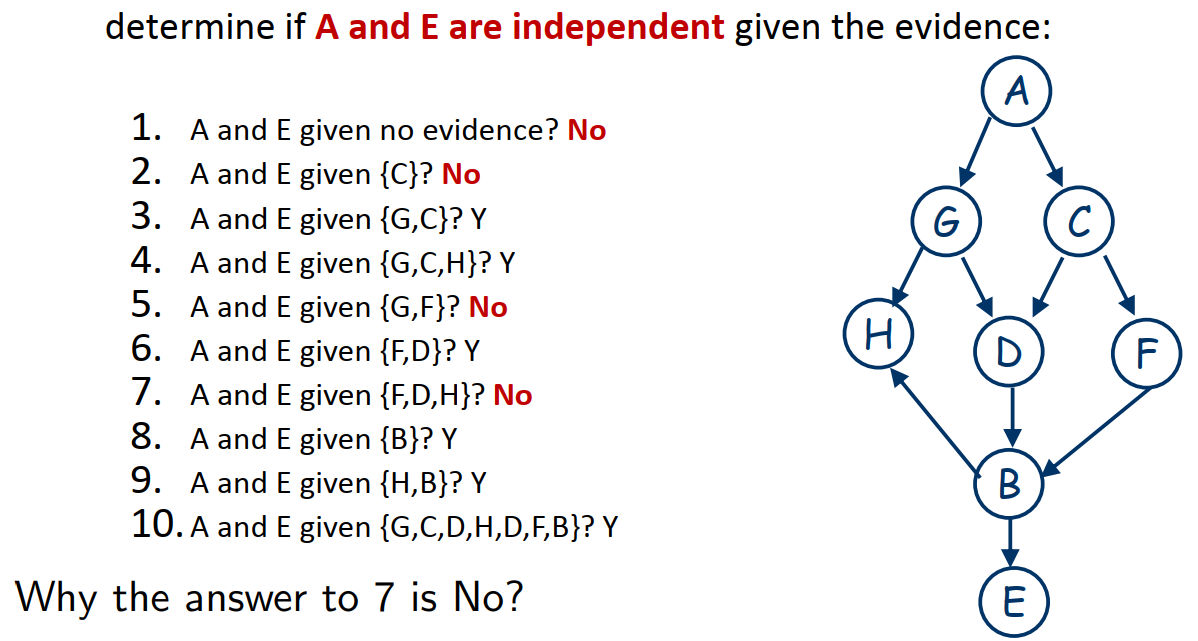
\includegraphics[width=0.8\linewidth]{fig/d-separation_example.png}
\end{figure}
注意第3种情况的适用条件,由于$H$在证据集中,所以并不满足第3种情况。
在第7个例子中,$AGHBE$没有被阻隔,故给定$FDH$,$A,E$也不独立。
\end{example}

\subsubsection{贝叶斯推断}
推断过程如下:
\[\begin{aligned}
\pr{a\mid d,e}&=\pr{a,d,e}/\pr{d,e}\\
&=\pr{a,d,e}/\sum_{A}\pr{a,d,e}\\
\pr{a,d,e}&=\sum_{B,C}\pr{a,B,C,d,e}
\end{aligned}\]
故只需计算$\pr{a,d,e}$。

采用动态规划的思想,存储子项,减少计算量。

记因子为某些变量的函数,如$\pr{C\mid A)}=f(A,C)$
\begin{itemize}
	\item 乘积:$h(X,Y,Z)=f(X,Y)\times g(Y,Z)$
	\item 求和:$h(Y)=\sum_{x\in\dom[X]}f(x,Y)$
	\item 因子限定:$h(Y)=f(a,Y)$
\end{itemize}

\begin{myalgorithm}[变量消除(Variable Elimination, VE)]
给定贝叶斯网络,条件概率表$F$,询问$Q$,证据$E$,其余变量为$Z$,计算$\pr{Q\mid E}$。
\begin{enumerate}
	\item 对于$f\in F$中每一变量,将其替换为$f_{E=e}$(因子限定)
	\item 对于每一$Z_j\in Z$,按给定$Z_j$顺序,并按照以下步骤消除:
	\begin{itemize}
		\item $f_1,f_2,\ldots,f_k$为含有$Z_j$的因子
		\item 计算新的因子$g_j=\sum_{Z_j}f_1\times f_2\times\cdots\times f_k$
		\item 将$f_i$从$F$中移除,并将新的因子$g_j$添加到$F$中
	\end{itemize}
	\item 剩下的因子只包含询问$Q$中的变量,则计算它们的乘积归一化得到$\pr{Q\mid E}$
\end{enumerate}
\end{myalgorithm}

可以采用桶消除(bucket elimination)算法,每次将新生成的因子放在第一个可被应用的桶中。
下图展示的是超图(hypergraph),最大超边(hyperedge)的大小即为最大的CPT表项/VE算法的复杂度。
\begin{figure}[H]
\centering
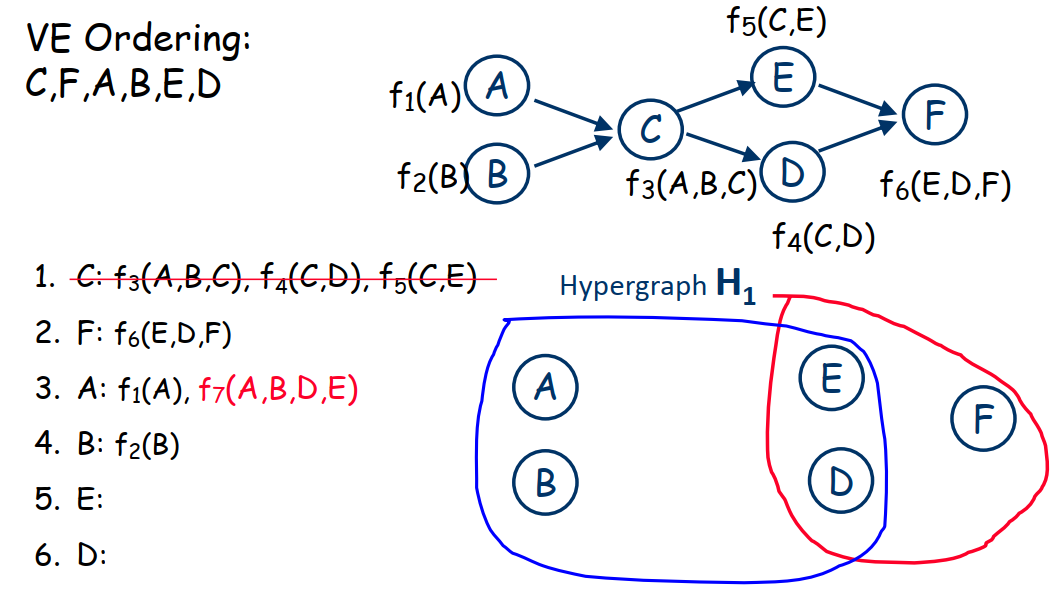
\includegraphics[width=0.8\linewidth]{fig/bucket_elimination.png}
\end{figure}

多树(polytree):单连通(singly connected)的贝叶斯网络,即在任意两个结点间只有一条路径。

最小填充(min-fill)启发式:总是先消除产生最小因子大小的变量,这种方法可以使得在线性时间内求解多树。

\begin{definition}[相关性(relevance)]
给定证据$E$询问$Q$,则有以下几种情况:
\begin{itemize}
	\item $Q$自身当然是相关的
	\item 若结点$Z$相关,则它的父母也相关
	\item 若$e\in E$是一个相关结点的\textcolor{red}{后代},则$E$也是相关的
\end{itemize}
\end{definition}
\begin{example}
\begin{figure}[H]
\centering
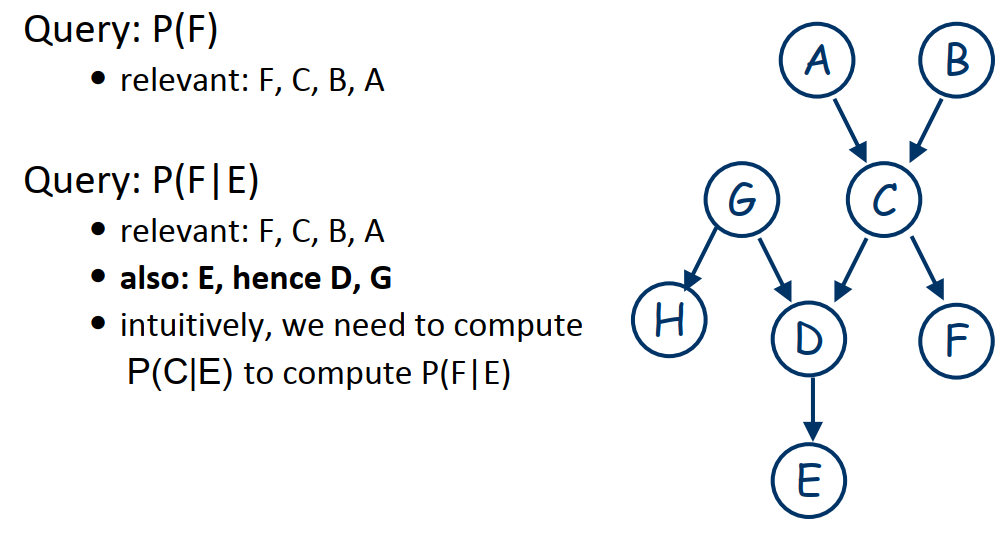
\includegraphics[width=0.8\linewidth]{fig/relevance_example.png}
\end{figure}
但询问$P(F\mid H)$,则$D,E,G$是不相关的。
而且这种算法会过度估计相关的变量。
\end{example}
% !TEX root = main.tex

\section{机器学习}
\subsection{决策树}
假定样本集合$D$中第$k$类样本所占比例为$p_k(k=1,2,\ldots,|\mathcal{Y}|)$,则$D$的信息熵定义为
\[\Ent(D)=-\sum_{k=1}^{|\mathcal{Y}|}p_k\log_2 p_k\]

又假定离散属性$a$有$V$个可能取值$\{a^1,a^2,\ldots,a^V\}$,第$v$个分支结点包含了$D$中所在属性$a$上取值为$a^v$的样本,记为$D^v$,进而可定义信息增益
\[\mathrm{Gain}(D,a)=\Ent(D)-\sum_{v=1}^V\frac{|D^v|}{|D|}\Ent(D^v)\]
每次选择最大增益的属性进行划分,即
\[a_*=\argmax_{a\in A}\mathrm{Gain}(D,a)\]

以信息增益为准则来选择划分属性的算法即为ID3决策树。

\subsection{贝叶斯学习}
先验$\pr{H}$、似然$\pr{d\mid H}$、证据$d=\lrang{d_1,d_2,\ldots,d_n}$,有贝叶斯公式(先验推后验)
\[\pr{H\mid d}=\alpha\pr{d\mid H}\pr{H}\]

假设独立同分布$\pr{d\mid h}=\prod_j\pr{d_j\mid h}$
\begin{itemize}
	\item 贝叶斯学习:$\pr{X\mid d}=\sum_i\pr{X\mid d,h_i}\pr{h_i\mid d}=\sum_i\pr{X\mid h_i}\pr{h_i\mid d}$
	\item 极大后验(MAP)学习:$\pr{X\mid d}\approx\pr{X\mid h_{MAP}}$
	\[h_{MAP}=\argmax_{h_i}\pr{h_i\mid d}=\argmax_{h_i}\pr{h_i}\pr{d\mid h_i}\]
	\item 最大似然(ML)学习:$\pr{X\mid d}\approx\pr{X\mid h_{ML}}$
	\[h_{ML}=\argmax_{h_i}\pr{d\mid h_i}\]
\end{itemize}

基于属性条件独立性假设
\[\pr{c\mid\vx}=\frac{\pr{c}\pr{\vx\mid c}}{\pr{x}}=\frac{\pr{c}}{\pr{\vx}}\prod_{i=1}^d\pr{x_i\mid c}\]
其中$d$为属性数目,$x_i$为$\vx$在第$i$个属性上的取值。
因对所有类别来说$\pr{\vx}$相同,因此贝叶斯判定准则为
\[h_{NB}(\vx)=\argmax_{c\in\mathcal{Y}}\pr{c}\prod_{i=1}^d\pr{x_i\mid c}\]
令$D_c$表示训练集$D$中第$c$类样本组成的集合,有
\[\pr{c}=\frac{D_c}{D}\qquad\pr{x_i\mid c}=\frac{|D_{c,x_i}|}{|D_c|}\]

\subsection{聚类算法}
\begin{itemize}
	\item 硬聚类:每个样本都决定放在哪一个类别中
	\item 软聚类:每个样本都被指派每个类别的概率分布
\end{itemize}

K-means算法
\begin{itemize}
	\item E步:对于每一个类别$i$和特征$X_j$,有
	\[pval(i,X_j)\gets\frac{\sum_{e:class(e)=i}val(e,X_j)}{|\{e:class(e)=i\}|}\]
	\item M步:对于每一个样本$e$,指派$e$给类别$i$使得
	\[\min_i\sum_{j=1}^n(pval(i,X_j)-val(e,X_j))^2\]
\end{itemize}

\subsection{神经网络}
\begin{theorem}[一致近似理论(Universal Approximator Theorem)]
具有至少一个隐层的深度神经网络可以无限逼近任意连续函数
\end{theorem}

前向后向传播过程:
\begin{itemize}
	\item 前向过程:
	\[in_j=\sum_i w_{ij}a_i\qquad a_j=g(in_j)\]
	\item 后向过程:
	\[\begin{aligned}
	\text{output:} & \Delta_j=g'(in_j)(y_j-a_j)\\
	\text{hidden:} & \Delta_i=g'(in_i)\sum_j w_{ij}\Delta_j
	\end{aligned}\]
\end{itemize}

注意以下两条求导公式
\[\begin{array}{rlrl}
\sigma(x)&=\dfrac{1}{1+\ee^{-x}} & \pd{\sigma(x)}{x}&=(1-\sigma(x))\sigma(x)\\
\tanh(x)&=\dfrac{\ee^x-\ee^{-x}}{\ee^x+\ee^{-x}} & \pd{\tanh(x)}{x}&=1-\tanh^2(x)
\end{array}\]

\subsection{强化学习}
目标:
\[\max_{\pi_\theta}\lrs{\sum_{t=1}^\infty\gamma^tr_t}\]

给定策略$\pi$:
\[\begin{aligned}
Q^\pi(s,a) &= \sum_{s'}\pr{s'\mid a,s}(R(s,a,s')+\gamma V^\pi(s'))\\
V^\pi(s) &= Q(s,\pi(s))
\end{aligned}\]

Q学习:随机选择动作$a$,观察回报$r$和下一状态$s'$
\[Q[s,a]\gets Q[s,a]+\alpha(r+\gamma\max_{a'}Q[s',a']-Q[s,a])\]

\end{document}